%==============================================================================
%  Individual differences in visual cortical representation decline along
%  the cortical hierarchy
%
%  Prepared for submission to Cerebral Cortex (Oxford University Press).
%
%  Cerebral Cortex asks for a single double-spaced file for review with tables
%  and figures embedded at their point of discussion, so this is a self-contained
%  manuscript. It compiles with pdfLaTeX on Overleaf as-is; OUP provides no class
%  file and does not require one.
%
%  Journal constraints enforced here (see wordcount.py and check_tex.py):
%    abstract <= 200 words, unstructured     keywords <= 5, alphabetical
%    main text <= 5000 words                 CSE name-year citations
%    section order: Intro, Materials and Methods, Results, Discussion,
%                   Acknowledgments, Funding, Conflict of Interest,
%                   Data Availability, Author Contributions, References
%
%  Compile: pdflatex -> bibtex -> pdflatex -> pdflatex
%==============================================================================
\documentclass[11pt,a4paper]{article}

\usepackage[T1]{fontenc}
\usepackage[utf8]{inputenc}
\usepackage{lmodern}
\usepackage{amsmath,amssymb}
\usepackage{graphicx}
\usepackage{booktabs}
\usepackage{siunitx}
\usepackage[margin=1in]{geometry}
\usepackage[hidelinks]{hyperref}
\usepackage{url}
\usepackage{authblk}
\usepackage{lineno}
\usepackage[font=small,labelfont=bf]{caption}
\usepackage{setspace}
\usepackage{natbib}
\bibliographystyle{apalike}
% Cerebral Cortex uses CSE name-year: "(Allen et al. 2022)", no comma before the
% year. The fifth argument of \bibpunct is that separator; apalike alone sets a
% comma. The reference list itself is restyled by OUP at production.
\bibpunct{(}{)}{;}{a}{}{,}

% Both locations are searched, so the figures work whether you upload the
% "figures" folder or drop the five PDFs loose into the project root.
\graphicspath{{figures/}{./}}

%--------------------------------------------------- reading copy vs review copy
% ONE switch controls line numbers and line spacing.
%
%   \reviewcopyfalse  clean copy: no line numbers, 1.5 spacing.
%                     Use this for reading and for your supervisor.
%
%   \reviewcopytrue   submission copy: continuous line numbers, double spacing,
%                     which is what Cerebral Cortex asks for.
%                     SWITCH THIS BACK ON BEFORE YOU SUBMIT.
%
\newif\ifreviewcopy
\reviewcopyfalse

\ifreviewcopy
  \linenumbers
  \doublespacing
\else
  \onehalfspacing
\fi

%------------------------------------------------------------------ title block
\title{\bfseries Shared visual representation increases along the ventral
hierarchy for semantic but not low-level features}

% Academic titles (Dr, Prof) are omitted from author lists by convention.
\author[1]{Daksh Kaila\thanks{Corresponding author:
\texttt{dkaila\_be25@thapar.edu}}}
\author[2]{Monika Aggarwal}
\affil[1]{Thapar Institute of Engineering and Technology, Patiala, Punjab, India}
\affil[2]{Indian Institute of Technology Delhi, New Delhi, India}
\date{}

\begin{document}
\maketitle

%---------------------------------------------------------------------- abstract
\begin{abstract}
\noindent
How much of a person's cortical representation of a natural scene is shared with
other people, and how much is theirs alone? We addressed this in the Natural
Scenes Dataset using the 766 images that all eight participants viewed at least
twice. Per-participant decoders mapped voxels into a common feature space, and we
asked how much of one participant's representation is recoverable from the other
seven, against a ceiling built from two decoders trained on disjoint halves of
each participant's images, so that decoder-specific error cancels. With a semantic target (CLIP), the recoverable fraction rose along the
ventral sequence from \num{0.835} in V1 to \num{0.948} in ventral stream in 8 of
8 participants ($\Delta = 0.113$, $t(7) = 7.29$, $p = 1.6\times10^{-4}$), and
survived matching regions for voxel count ($\Delta = 0.093$, $p = 0.022$). With a
low-level target (GIST) the same voxels showed no gradient (V1 \num{0.889},
ventral stream \num{0.883}; $\Delta = -0.006$, $p = 0.89$), and equivalence
testing excluded a semantic-sized effect; this was not weaker decoding, as GIST
identification exceeded CLIP in V1. The region-by-target interaction was reliable
($t(7) = 3.02$, $p = 0.020$). A decoder-free measure of representational
geometry placed V1 sixth from the bottom of sixteen regions. Where visual representation is individual therefore depends on the
feature space in which it is measured.
\end{abstract}

\vspace{0.5em}
\noindent\textbf{Keywords:} individual differences; inter-subject decoding;
Natural Scenes Dataset; representational similarity analysis; visual cortex

\clearpage

%------------------------------------------------------------------ introduction
\section{Introduction}

Functional neuroimaging routinely averages across participants, an operation that
presupposes a representational code common enough for averaging to be meaningful.
Where that presupposition holds, and where it fails, is a quantitative question
that has been difficult to answer because two very different situations look
alike in the data: a region may fail to generalise across people because its code
is genuinely individual, or because it carries too little reliable signal for any
comparison to succeed. Distinguishing them requires an explicit noise ceiling
\citep{nili2014,walther2016,lagecastellanos2019}, and much prior work on
inter-subject representational similarity reports raw alignment without one.

The question is not whether brains differ. Individual differences in functional
organisation are large, stable and measurable, whether indexed by connectivity
fingerprints that identify a person across sessions \citep{finn2015}, by the
areal layout of a densely sampled individual \citep{laumann2015,wang2015}, or by
the finding that stable individual factors dominate day-to-day variation in
functional networks \citep{gratton2018}. What is unsettled is where in the visual
hierarchy those differences reside in the \emph{content} of a representation, as
opposed to its spatial arrangement, and how to measure that without mistaking
unreliability for individuality \citep{dubois2016,seghier2018}.

Representational similarity analysis \citep{kriegeskorte2008} provides a natural
vocabulary for this question, since representational dissimilarity matrices are
defined over stimuli rather than voxels and are therefore comparable across
brains without spatial correspondence. \citet{charest2014} showed that individual
differences in such geometry are behaviourally meaningful, predicting each
person's own perceived similarity judgements. That work established that
individuality in representation is real; here we ask where along the cortical
hierarchy it resides, and how much of it each region carries once measurement
noise is accounted for.

Functional alignment methods, including hyperalignment \citep{haxby2011}, searchlight
hyperalignment \citep{guntupalli2016} and the shared response model
\citep{chen2015}, demonstrate that a common space can be recovered across
participants, and are typically evaluated by how much they improve cross-subject
classification. Hyperalignment also makes fine-grained individual differences
more reliably measurable than anatomical normalisation allows
\citep{feilong2018}, and shared-subject decoding models now exploit this to
reconstruct images in a new participant from an hour of data
\citep{scotti2024}. That framing answers a different question from ours. We are
not asking how well brains \emph{can} be aligned given a flexible transform, but
how much of each region's representational content is \emph{already} common when
stimulus identity alone provides the correspondence.

The Natural Scenes Dataset \citep{allen2022} makes this tractable. Its 1{,}000
\emph{shared} images were viewed by all participants, supplying a
stimulus-identity correspondence that requires no spatial alignment, and its
extensive scale (up to 40 sessions per participant) supplies enough data to train
per-participant decoders and to measure within-participant reliability directly
rather than assuming it. Decoding voxels into an image-computable feature space is
a standard way to make brains comparable \citep{naselaris2011,kay2008,kamitani2005,
horikawa2017}, and vision-language embeddings in particular predict high-level
visual cortex well \citep{radford2021,wang2023}, which is also why we test a
low-level feature space alongside them.

We ask three questions. Which regions represent natural scenes in a form that
transfers between brains? Where does that transfer break down, once bounded by
each region's own reliability and measured against a ceiling that shares no
decoder with the quantity it bounds? And does the answer depend on the feature
space the representation is read out into? The third question turns out to decide
the first two.

%----------------------------------------------------------- materials and methods
\section{Materials and Methods}

\subsection{Data}

We used the Natural Scenes Dataset \citep{allen2022}, 7T fMRI at 1.8\,mm
isotropic resolution. All eight participants were included: four completed 40
scan sessions, two completed 32, and two completed 30, giving 284 sessions and
213{,}000 stimulus trials in total. Analyses used the
\texttt{betas\_fithrf\_GLMdenoise\_RR} single-trial GLM estimates in each
participant's native functional space (\texttt{func1pt8mm}).

Stimulus identity was recovered from each participant's behavioural log as
$\mathrm{nsdId} = \mathrm{73KID} - 1$. This relation was verified three ways: the
shared-image index set matched only under the offset; every one of a
participant's unique images fell within their assigned image set only under the
offset; and the dataset's own first-presentation trial indices matched the
observed presentation order only under the offset. We note this because an
off-by-one error here is silent, assigning each trial the annotations of a
different photograph, and we found such an error in an earlier analysis
pipeline applied to these data.

\subsection{Regions of interest}

Twenty-one regions were extracted per participant from the dataset's own
definitions: V1, V2, V3 and hV4 from \texttt{prf-visualrois}; FFA from
\texttt{floc-faces}; OPA, PPA and RSC from \texttt{floc-places}; perirhinal,
entorhinal and parahippocampal cortex, subiculum, CA1 and DG/CA3 from the
high-resolution medial temporal segmentation; the six-way \texttt{streams}
parcellation of visual cortex; and \texttt{nsdgeneral}. Label assignments follow
the dataset documentation; we flag that \texttt{prf-visualrois} labels 1--4
denote V1v, V1d, V2v and V2d rather than V1--hV4, and that \texttt{floc-places}
label 1 is OPA rather than PPA. Dorsal and ventral halves were pooled, so V1 is
the union of labels 1 and 2, V2 of labels 3 and 4, V3 of labels 5 and 6, and hV4
is label 7.

Responses were $z$-scored per voxel within scan session before analysis. This is
the minimum defensible normalisation for an experiment spanning roughly nine
months per participant.

\subsection{Test set}

All analyses were evaluated on the 766 shared images that every participant
viewed at least twice. Requiring two viewings permits a within-participant
reliability estimate computed from independent presentations, which serves as the
noise ceiling throughout.

\subsection{Measure 1: shared representational geometry}

For each region and participant we computed a $766 \times 766$ representational
dissimilarity matrix (RDM, correlation distance) separately from the first and
second presentation of each image. Within-participant reliability
$r_{\mathrm{within}}$ is the correlation between those two RDMs.
Between-participant similarity $r_{\mathrm{between}}$ is the mean correlation
between one participant's RDM and another's.

Critically, $r_{\mathrm{between}}$ uses \emph{crossed} presentation pairings only
(participant $s$'s first presentation against participant $o$'s second, and vice
versa), matching the structure of $r_{\mathrm{within}}$. Including matched
pairings gives $r_{\mathrm{between}}$ an advantage that $r_{\mathrm{within}}$
cannot have whenever presentation order carries any systematic effect, and
inflates the ratio above its bound. The shared fraction is
\begin{equation}
\mathrm{shared} = \frac{r_{\mathrm{between}}}{r_{\mathrm{within}}},
\label{eq:shared}
\end{equation}
which is 1 when all reliable geometry is common across brains and 0 when it is
entirely individual.

Equation~\ref{eq:shared} divides by participant $s$'s own reliability rather than
by the symmetric disattenuation $\sqrt{r_{\mathrm{within},s}\,
r_{\mathrm{within},o}}$ \citep{walther2016,lagecastellanos2019}. The two answer
different questions: the symmetric form estimates the correlation between two
noise-free RDMs, whereas Equation~\ref{eq:shared} is directional and asks what
fraction of \emph{this} participant's reliable geometry another brain recovers,
which is the quantity this paper is about. The choice also matters empirically.
Because $r_{\mathrm{within}}$ varies up to 26-fold across participants in the
least reliable regions, the symmetric normaliser would scale estimates by a
factor that ranges from \num{1.024} (V1) and \num{1.024} (V2) to \num{1.305}
(parietal stream), and would place four regions above 1 --- impossible for a
shared fraction. The regions this paper interprets are the least affected, and
the ordering at the extremes is unchanged.

\subsection{Measure 2: transfer in a common embedding space}

Representational geometry describes relations among stimuli; it does not describe
the representation of any individual stimulus. For a per-image measure we mapped
every participant's voxels into one common space.

For each participant and region we trained ridge regression
\citep{naselaris2011} from voxels to the 768-dimensional CLIP ViT-L/14 image
embedding \citep{radford2021} of the viewed stimulus. Training used only that
participant's \emph{own} non-shared images (8{,}302--9{,}000 images, roughly
24{,}000 trials); the 766 shared images were never seen during training. Voxels
were reduced by PCA to 1{,}000 components fitted on training images alone, so
that no test structure entered the basis. The regularisation parameter was
selected by five-fold cross-validation within the training set.

After decoding, all eight participants yield comparable 768-dimensional vectors
for the same photograph, and the mismatch between their voxel spaces becomes
irrelevant. Leaving out one participant at a time, we compared their decoded
embedding for each shared image against each of the other seven participants'
decoded embedding of the same image, and averaged the seven resulting cosine
similarities.

We average on the similarity scale rather than averaging the seven embeddings
first, and this choice is not cosmetic. Averaging embeddings would reduce noise
on the predictor side alone, leaving the numerator with a cleaner predictor than
the single-presentation ceiling in the denominator, and the ratio would then
exceed 1 for arithmetic rather than neurobiological reasons. Every cosine
entering the numerator therefore compares one presentation of one participant
against one presentation of one other participant, matching the structure of the
ceiling exactly. The quantity we report is accordingly how much of a
participant's representation is recoverable from a \emph{typical other brain},
not from an optimally pooled seven-participant estimate; the latter would be a
larger number and would not be comparable to this ceiling.

Two corrections are essential. First, ridge shrinks predictions toward the
training centroid, so predictions for entirely different images already sit at
cosine 0.93--0.996; all cosines are therefore computed after removing the
across-image mean, leaving only the stimulus-varying component. Second, model
selection used two-way identification accuracy rather than raw cosine, because
raw cosine is maximised by collapsing every prediction onto the centroid and
therefore selects the most over-regularised model.

Cosines are computed after subtracting the across-image mean from each set of
predictions separately. The mean is taken over the 766 test images of that set,
within participant and region, and never from training predictions. Without this
step ridge shrinkage leaves predictions for unrelated images at cosines above
\num{0.9}, so the raw cosine compares two near-identical mean vectors rather than
anything stimulus-specific.

Transfer and ceiling are matched for noise: both compare one presentation against
one other presentation, using crossed pairings, so their ratio is interpretable.
Per-image ratios are not computed because the denominator crosses zero for individual
images; the participant is therefore treated as the unit of analysis, and the ratio is
computed once per participant from their image-averaged cosines.

\subsection{Interpretability gating}

Transferability is bounded by reliability. A region whose decoded representations
do not identify the viewed image cannot support a transfer measurement, and its
transfer/ceiling ratio is one noise estimate divided by another. We therefore
required within-participant two-way identification accuracy of at least 0.55
(chance 0.5), a criterion analogous in spirit to the noise ceiling of
\citet{nili2014} but expressed on a scale with a known chance level. Regions
failing this criterion are reported as underpowered, not as individual: at that
signal level the two are indistinguishable.

\subsection{Control analyses}

Three controls test whether the transfer gradient is a property of cortex or of
the way it is measured. All three are reported whatever their outcome.

\emph{A decoder-independent ceiling.} The ceiling defined above compares one
decoder's output on two presentations. Both sides therefore run through the same
ridge model, the same basis and the same training images, so any error that model
makes which depends on the image is identical on both sides and inflates the
ceiling, whereas transfer compares two different participants' decoders and that
shared error cancels. The inflation should be largest where the voxel-to-embedding
mapping is weakest, which is early visual cortex against a semantic target --- the
pattern we report. We therefore split each participant's training images into two
disjoint halves and fitted two decoders, $A_s$ and $B_s$, with independent bases.
The ceiling becomes the mean of $\cos(A_s(p_1), B_s(p_2))$ and
$\cos(B_s(p_1), A_s(p_2))$, and transfer the same expression with $B_o$ and $A_o$
in place of $B_s$ and $A_s$. Numerator and denominator are then matched in
training-set size, in decoder independence and in presentation count, leaving same
brain versus different brain as the only difference. The split is by image, not by
trial: each non-shared image is presented about three times, so splitting by trial
would leave both decoders sharing image-specific information.

\emph{A low-level target.} A semantic target can make high-level regions look
shared by construction. We repeated the entire analysis with a 512-dimensional
GIST descriptor \citep{oliva2001} --- four spatial scales by eight orientations of
Gabor energy over a $4\times4$ grid, a V1-like model with no semantic content ---
in place of the CLIP embedding.

\emph{Matched region size.} Regions differ in voxel count by a factor of 30. Every
region was subsampled to the smallest analysed region's voxel count for that
participant (397--566 voxels), with three independent random subsamples averaged,
and the split-half analysis repeated.

\subsection{Image categories}

Each shared image was assigned to its COCO supercategory \citep{lin2014}, taking
the most frequent supercategory among its object annotations. Twelve
supercategories were represented among the 766 test images, ranging from 187
images (\emph{person}) to 15 (\emph{sports}). Because the spread of a set of
category means grows with the noise in those means, the observed spread was
compared against a null built by permuting the image-to-category assignment 500
times and recomputing every region's spread.

\subsection{Statistics}

Contrasts between regions are paired $t$-tests across the eight participants,
each participant contributing one value per region. Contrasts against V1 were
corrected for multiple comparisons across the 15 remaining regions using the
Benjamini--Hochberg procedure; both raw and adjusted values are reported.
Permutation nulls, shuffling image identity for one participant, were computed
for every region.

\subsection{Validation}

Stimulus images were verified by full decode (not header read), geometry and
non-blankness; all 70{,}566 passed. Embedding extraction aborts on non-finite or
stimulus-invariant features. Stimulus ordering between brain and model
representations is asserted rather than assumed. Every number in the figures and
tables below is regenerated from the trial-level result files by the analysis
scripts and checked against the stored per-region summaries before the manuscript
is built; that check is part of the released code.

%----------------------------------------------------------------------- results
\section{Results}

\subsection{Shared representational geometry}

Permutation nulls were at zero for all 21 regions (maximum absolute deviation
\num{0.0005}), confirming that cross-participant correspondence, rather than RDM
structure, drives the measured alignment.

Among regions with usable reliability, the shared fraction ranged from
\num{0.611} in hV4 to \num{0.971} in ventral stream (Table~\ref{tab:main}).
Departures from a fully shared code survived Benjamini--Hochberg correction
across the 16 regions \citep{benjamini1995} in early and mid-level visual cortex
(hV4: $p = 5.6\times10^{-4}$, $q = 5.6\times10^{-4}$; V1: $p = 0.003$,
$q = 0.004$; V2: $p = 0.004$, $q = 0.004$; mid-ventral stream: $p = 0.005$,
$q = 0.007$; parietal stream: $p = 0.009$, $q = 0.013$; V3: $p = 0.027$,
$q = 0.041$). Scene-selective and ventral-stream regions were not significantly
below 1. With eight participants and standard errors near \num{0.10} this is
absence of evidence for an individual component, not evidence that these codes
are completely shared.

\subsection{Transfer in the common embedding space}

All sixteen regions with usable decoders cleared the identification criterion
(within-participant identification \num{0.675}--\num{0.962}; chance \num{0.5};
Figure~\ref{fig:ident}A) and all showed transfer far above zero (all
$p < 10^{-6}$; Table~\ref{tab:main}).

The fraction of a participant's own decodable representation recoverable from the
other seven increased with distance from primary visual cortex (V1: \num{0.715};
V2: \num{0.750}; V3: \num{0.829}; hV4: \num{0.833}), continuing through
mid-level streams (\num{0.859}--\num{0.861}) and scene- and face-selective
cortex (\num{0.893}--\num{0.911}) to ventral stream (\num{0.933};
Figure~\ref{fig:gradient}, Table~\ref{tab:main}).

Because the 16 regions overlap and are nested, and mix dorsal with ventral
areas, a group-mean ranking over all of them does not test a hierarchy. We
therefore pre-specified one ordered ventral sequence (V1 $\rightarrow$ V2
$\rightarrow$ V3 $\rightarrow$ hV4 $\rightarrow$ mid-ventral $\rightarrow$
ventral stream) and fitted a linear slope per participant across its six
positions. The slope was positive in 8 of 8 participants (mean
\num{0.041} per step, $t(7) = 14.67$, $p = 1.6\times10^{-6}$, $d_z = 5.19$). The
increase is therefore reliable but not strictly monotonic: no participant's
sequence is ordered without a single inversion (mean Kendall
$\tau = \num{0.783}$, $t(7) = 11.80$, $p = 7.1\times10^{-6}$), most often hV4
falling below V3. We describe the sequence as rising, not as monotonic.

The ordering is not an artefact of differing signal quality: the same gradient is
present in the raw transfer cosines and in the ceilings separately
(Figure~\ref{fig:gradient}B), and V1's ceiling is among the highest in the
dataset. Nor does it track region size: voxel counts differ by a factor of 30 but
correlate only weakly with transfer ($r = \num{0.358}$, $p = 0.174$ on
$\log_{10}$ voxels), and hV4, the smallest region we analyse (\num{498} voxels),
transfers at \num{0.833}, well above V1 (\num{1130} voxels, \num{0.715}). A
direct subsampling control is reported below.
The number of scanning sessions, which varies from 30 to 40 between participants,
is also not responsible: it is a between-participant quantity and cannot generate
a difference between regions within a participant, and across participants it is
if anything negatively related to mean transfer ($r = -0.641$, $p = 0.087$).

\begin{figure}[tb]
\centering
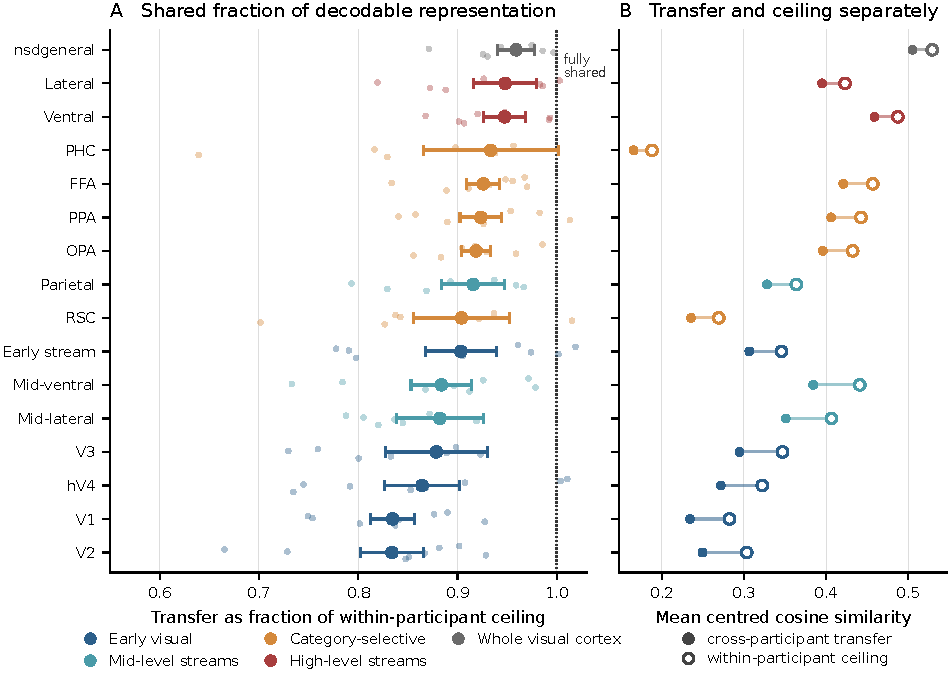
\includegraphics[width=\textwidth]{fig1_gradient.pdf}
\caption{\textbf{Representational transfer between brains increases along the
cortical hierarchy.}
\textbf{(A)} For each region, the fraction of a participant's own decodable
representation that is recoverable from the other seven participants. Large
symbols are the group mean with standard error over the 8 participants; small
translucent points are individual participants. The dotted line at 1 marks a
fully shared code. Colour denotes hierarchical tier.
\textbf{(B)} The two quantities whose ratio forms panel A, plotted separately:
cross-participant transfer (filled) and within-participant ceiling (open), both
as mean-centred cosine similarity. Regions differ widely in absolute signal, yet
the ordering in panel A does not follow that of the ceiling; V1 is neither
the noisiest nor the weakest region, but it is the least transferable.
Region order is identical in both panels.}
\label{fig:gradient}
\end{figure}

Within-participant contrasts against V1 were large and consistent
(Table~\ref{tab:contrast}). Ventral stream exceeded V1 by
$\Delta = \num{0.218}$ ($t(7) = 17.19$, $p = 5.5\times10^{-7}$,
$q = 4.2\times10^{-6}$), and every one of the eight participants showed the
effect in the same direction (Figure~\ref{fig:paired}A). All 15 contrasts against
V1 survived Benjamini--Hochberg correction, 14 of them at $q < 0.01$. The sole
marginal comparison is V2 versus V1 ($\Delta = \num{0.035}$, $t(7) = 2.45$,
$q = 0.044$, 6 of 8 participants), which is expected given that V1 and V2 are
adjacent in the hierarchy and is the one step in the gradient we would not claim
on this evidence alone.

Individual participants vary considerably in the absolute level of transfer, and
in the least reliable regions the per-participant estimates are noisy
(Figure~\ref{fig:paired}B). The V1-to-ventral gradient itself, however, is
recovered in every participant separately.

\begin{figure}[tb]
\centering
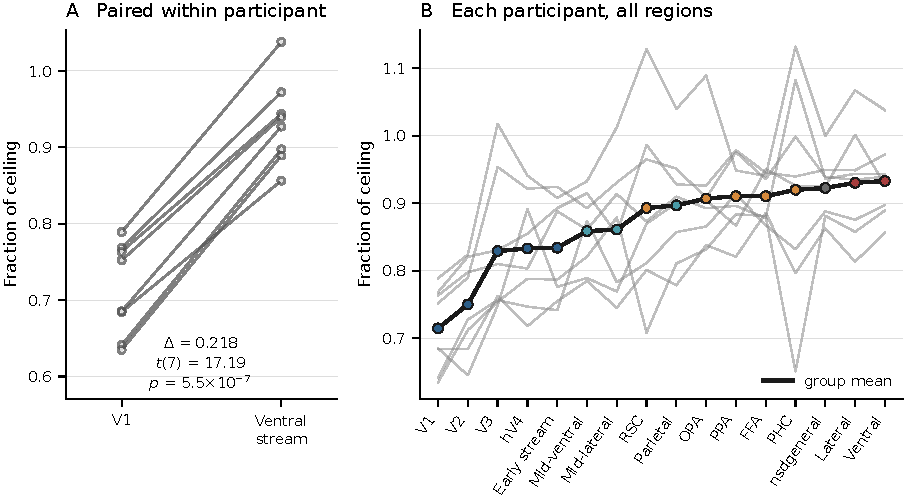
\includegraphics[width=\textwidth]{fig2_per_participant.pdf}
\caption{\textbf{The gradient holds in every participant.}
\textbf{(A)} Transfer as a fraction of ceiling in V1 and in ventral stream, one
line per participant. All eight participants show higher transfer in ventral
stream; none is an exception. Statistics are a paired $t$-test across the eight
participants.
\textbf{(B)} The full per-participant profile across all sixteen regions, ordered
by group mean (grey lines, individual participants; black line with coloured
markers, group mean). The spread widens in regions with lower reliability, most
conspicuously parahippocampal cortex, whose individual estimates range from
below \num{0.65} to above \num{1.1}, reflecting the expected behaviour of a ratio
of two noise estimates and justifying treating that region as unstable throughout.}
\label{fig:paired}
\end{figure}

\subsection{What the gradient depends on}

Three controls were applied to the pre-specified ventral sequence, each reported
whatever its outcome. All use the split-half ceiling, so the numerator and
denominator are matched in training-set size, decoder independence and
presentation count.

\emph{The ceiling was inflated, and the gradient is half its apparent size.}
Comparing one decoder's output across two presentations overstates
within-participant agreement, and it does so most where the voxel-to-embedding
mapping is weakest: the ceiling falls by \num{0.081} in V1 but only \num{0.029}
in mid-ventral cortex when the two sides are given independent decoders. The
gradient therefore shrinks by about half. The shared fraction rises from
\num{0.835} in V1 to \num{0.948} in ventral stream, a gap of \num{0.113} against
\num{0.218} uncorrected ($t(7) = 7.29$, $p = 1.6\times10^{-4}$, $d_z = 2.58$, 8
of 8 participants), and the per-participant slope falls from \num{0.055} to
\num{0.028} per step ($t(7) = 7.32$, $p = 1.6\times10^{-4}$). The effect is
smaller than we first measured but it is not an artefact of the ceiling.

\emph{Region size does not explain it.} Subsampling every region to the smallest
region's voxel count for that participant leaves the gap essentially intact
(\num{0.093}, $t(7) = 2.94$, $p = 0.022$, $d_z = 1.04$; slope \num{0.025} per
step, positive in 8 of 8). Matching for size costs little beyond the ceiling
correction itself.

\emph{The gradient is specific to a semantic target.} Repeating the analysis with
a GIST descriptor in place of the CLIP embedding removes it. The shared fraction
is \num{0.889} in V1, \num{0.893} in V2, \num{0.842} in hV4, \num{0.837} in
mid-ventral cortex and \num{0.883} in ventral stream: a V1-to-ventral gap of
$-\num{0.006}$ ($t(7) = -0.15$, $p = 0.89$, positive in 3 of 8 participants) and
a slope indistinguishable from zero ($-\num{0.007}$ per step, $p = 0.48$). This
is an informative null rather than a failure to detect. The \SI{95}{\percent}
confidence interval on the GIST gap, $[-\num{0.100}, +\num{0.088}]$, excludes the
semantic gap of \num{0.113}, and two one-sided tests against that bound support
equivalence ($p = 0.015$ and $p = 0.010$). Nor is it weak decoding: GIST
identification was above chance in every region (\num{0.744}--\num{0.875}) and
\emph{exceeded} CLIP identification in V1 (\num{0.875} versus \num{0.793},
$t(7) = 8.38$, $p < 0.001$), while the GIST ceiling in V1 was nearly twice the
CLIP ceiling (\num{0.525} versus \num{0.282}). Early visual cortex is the region
where the low-level target works best, and it is also where the two targets
disagree most about how shared the representation is. The region-by-target
interaction is reliable (\num{0.119}, $t(7) = 3.02$, $p = 0.020$, same sign in 7
of 8 participants).

Taken together, the hierarchy gradient we set out to measure holds for semantic
content and does not hold for low-level content in the same voxels. We therefore
report it as a property of the semantic read-out rather than of the cortical
hierarchy as such.

\subsection{Convergence between measures}

The two measures agree in rank ordering (Spearman $\rho = 0.556$, $p = 0.025$
across 16 regions) but not in magnitude (Pearson $r = 0.350$, $p = 0.183$;
Figure~\ref{fig:cross}). The agreement is carried by the ends of the ranking.
Both place ventral stream among the most shared regions, and both place V1 and V2
in the lower half, but neither the geometry measure nor the decoding measure puts
early visual cortex lowest overall: by geometry V1 ranks sixth of 16 from the
bottom, behind hV4 (\num{0.611}), mid-ventral (\num{0.653}), parietal
(\num{0.660}) and mid-lateral stream (\num{0.702}). Excluding parahippocampal
cortex, whose reliability is lowest and whose estimate is the largest single
disagreement, rank agreement rises to $\rho = \num{0.746}$ ($p = 0.001$, 15
regions). Several intermediate regions diverge substantially
(e.g., hV4 is \num{0.833} by decoding but \num{0.611} by geometry). We therefore
treat the \emph{ordering} as the replicated result and do not claim quantitative
agreement between the two measures.

\begin{figure}[tb]
\centering
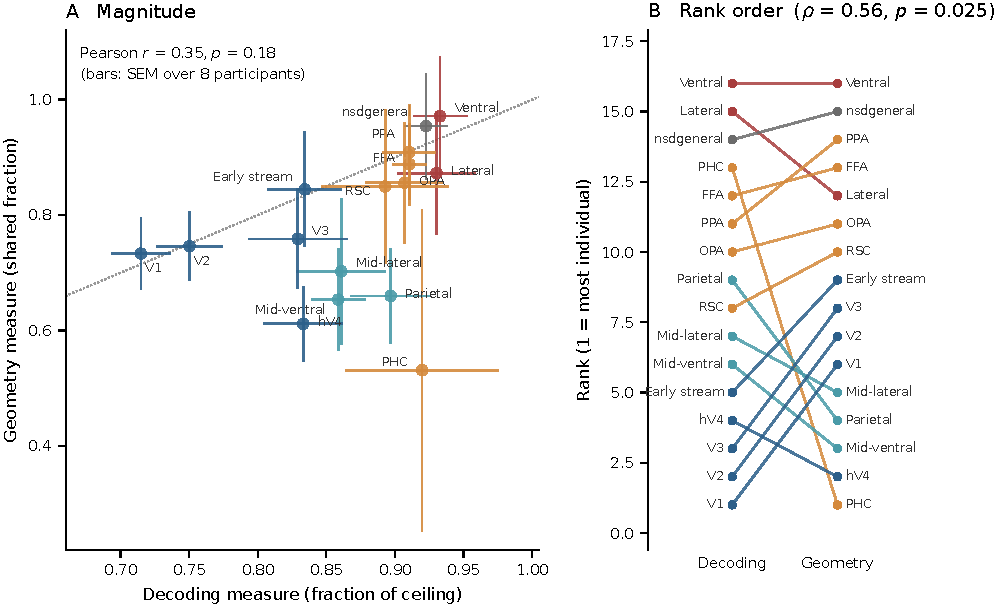
\includegraphics[width=\textwidth]{fig3_cross_method.pdf}
\caption{\textbf{The two measures replicate each other's ordering, not their
magnitudes.}
\textbf{(A)} Geometry-based shared fraction against decoding-based fraction of
ceiling, one point per region; bars are standard errors over the 8 participants
and the dotted line is the identity. The correlation in magnitude is not
significant.
\textbf{(B)} The same 16 regions ranked by each measure (rank 1 = most
individual). The two extremes agree; intermediate regions reorder.
Parahippocampal cortex is the largest disagreement, consistent with its low
reliability under both measures.}
\label{fig:cross}
\end{figure}

\subsection{Dependence on image category}

Transfer in V1 varied across COCO supercategories \citep{lin2014} over a wider
range than transfer in ventral stream (V1 range \num{0.625}--\num{0.803}, span
\num{0.178}; ventral stream \num{0.886}--\num{0.966}, span \num{0.079};
Figure~\ref{fig:category}, Table~\ref{tab:category}). In V1, images of food
(\num{0.803}) and vehicles (\num{0.799}) transferred best while furniture
(\num{0.625}) and kitchen objects (\num{0.655}) transferred worst.

This difference in span is not interpretable. The span of a set of category means
grows with the noise in those means, and V1 has both the lowest transfer and the
smallest categories (15 images for \emph{sports}). A null built by permuting the
image-to-category assignment 500 times produces a V1-to-ventral span ratio
\emph{larger} than the one observed (observed \num{2.24}, null mean \num{2.77},
$p = 0.641$). We draw no inference from the category results.

\begin{figure}[tb]
\centering
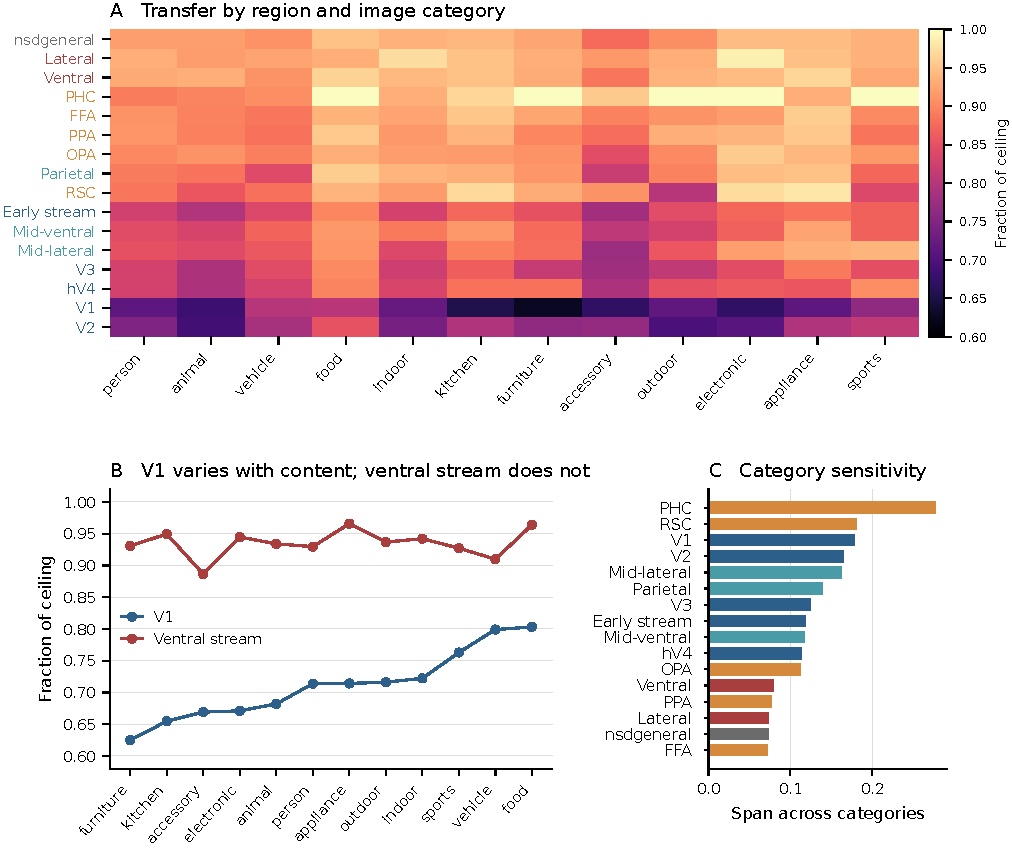
\includegraphics[width=\textwidth]{fig4_category.pdf}
\caption{\textbf{Transfer by image category, which a permutation null shows to be
uninformative.}
\textbf{(A)} Fraction of ceiling for each region (rows, ordered as in
Figure~\ref{fig:gradient}) and COCO supercategory (columns, ordered by number of
images). Colour is clipped at 1.0; parahippocampal cortex exceeds this for one
category (\emph{outdoor}, \num{1.170}), which is not physically interpretable
and reflects that region's low reliability.
\textbf{(B)} V1 and ventral stream plotted against category, with categories
ordered by V1 transfer. V1 spans \num{0.178}; ventral stream spans \num{0.079}.
\textbf{(C)} Span across categories for every region. The largest spans are in
RSC and early visual cortex and the smallest in ventral, lateral and
face-selective cortex, but this ordering tracks each region's noise rather than
its category sensitivity and we draw no inference from it.}
\label{fig:category}
\end{figure}

\subsection{The same result on an identification scale}

On an identification scale the gradient is not driven by regions differing in how
much stimulus information they carry. Accuracy from a participant's own decoder
was high throughout (\num{0.675}--\num{0.962}), and the within- minus
cross-participant gap is largest where transfer is lowest: \num{0.081} in V1
against \num{0.016} in ventral stream (Figure~\ref{fig:ident}B), and likewise
\num{0.044} against \num{0.014} under the split-half decoders. V1's
stimulus-specific information is decodable within a participant; less of it
generalises. This is a rescaling of the same quantity, not independent evidence
--- the gap and the transfer ratio correlate at $r = -\num{0.993}$ across the 16
regions --- and we report it only because identification has a known chance level
and no dependence on the centring convention.

\begin{figure}[tb]
\centering
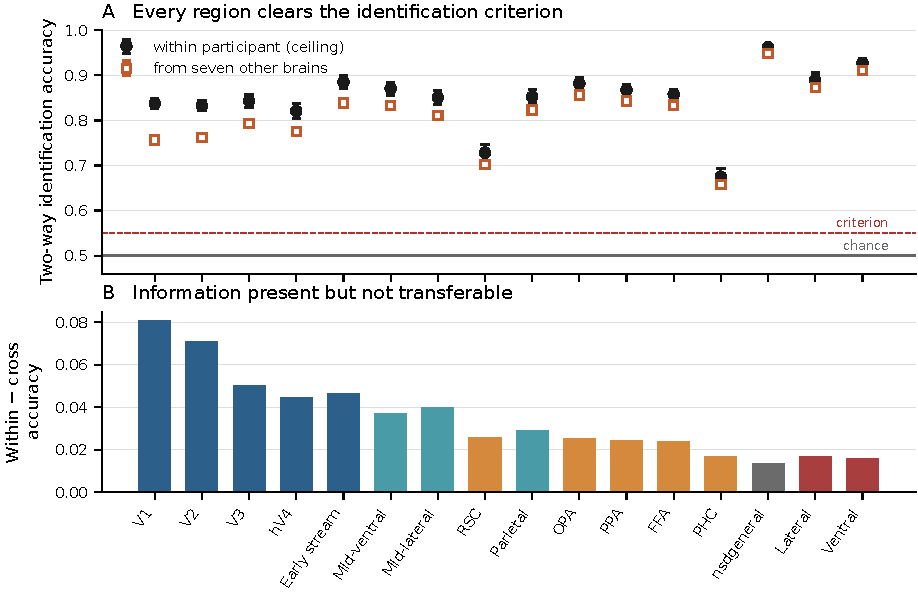
\includegraphics[width=\textwidth]{fig5_identification.pdf}
\caption{\textbf{Identification accuracy confirms that low transfer is not low
signal.}
\textbf{(A)} Two-way identification accuracy (chance \num{0.5}) for each region,
computed within participant from their own decoder (filled) and, averaged over
the seven other participants, from each of their decoders in turn (open). Error
bars are standard errors over the 8 participants. Every region clears the \num{0.55} criterion required for its
transfer ratio to be interpretable.
\textbf{(B)} The difference between the two, by region, in the same order. The
gap is widest in V1 and V2 and narrowest in ventral and lateral stream: early
visual cortex carries as much decodable stimulus information as anywhere else,
but less of it is recoverable from other brains.}
\label{fig:ident}
\end{figure}

\subsection{Regions that cannot be assessed}

Within-participant RDM reliability was at floor in perirhinal cortex
(\num{0.0014}), subiculum (\num{0.0008}), CA1 (\num{0.0007}) and DG/CA3
($-\num{0.0004}$); entorhinal cortex was only marginally above it
(\num{0.0171}) (Table~\ref{tab:excluded}). At this level, a region's code being
individual and a region carrying no measurable code are mathematically
indistinguishable, and we make no claim about these structures. Parahippocampal
cortex cleared the identification criterion but only marginally (\num{0.675}, the
lowest of the sixteen, with the largest standard error), produced a
category-wise estimate above 1 (Figure~\ref{fig:category}A), and disagreed most
strongly between the two measures (Figure~\ref{fig:cross}B); we regard its
estimate as unstable and exclude it from the interpretation.

%------------------------------------------------------------------------ tables
\begin{table}[tb]
\centering
\caption{\textbf{Shared representation by region, both measures.} \emph{Transfer}
is the decoding-based fraction of the within-participant ceiling, with its
standard error over the 8 participants. \emph{Ident.\ within} and \emph{Ident.\
cross} are two-way identification accuracy (chance \num{0.5}) from a
participant's own decoder and, averaged over the seven other participants, from
each of their decoders in turn. \emph{Shared} is
the geometry-based fraction of Equation~\ref{eq:shared} with its standard error,
and the final column tests it against 1 (a fully shared code); it is not reported
for parahippocampal cortex, whose within-participant RDM reliability falls below
the threshold at which the ratio is meaningful. Regions are ordered by transfer.}
\label{tab:main}
\small
\begin{tabular}{lccccccc}
\toprule
 & \multicolumn{4}{c}{Decoding measure} & \multicolumn{3}{c}{Geometry measure} \\
\cmidrule(lr){2-5}\cmidrule(lr){6-8}
Region & Transfer & SEM & Ident.\ within & Ident.\ cross & Shared & SEM & $p$ vs.\ 1 \\
\midrule
Ventral stream      & \num{0.933} & \num{0.020} & \num{0.927} & \num{0.911} & \num{0.971} & \num{0.103} & 0.786 \\
Lateral stream      & \num{0.930} & \num{0.029} & \num{0.889} & \num{0.872} & \num{0.872} & \num{0.107} & 0.275 \\
nsdgeneral          & \num{0.923} & \num{0.016} & \num{0.962} & \num{0.949} & \num{0.954} & \num{0.092} & 0.630 \\
Parahippocampal     & \num{0.920} & \num{0.056} & \num{0.675} & \num{0.658} & \num{0.531} & \num{0.279} & --- \\
FFA                 & \num{0.911} & \num{0.012} & \num{0.858} & \num{0.834} & \num{0.888} & \num{0.071} & 0.157 \\
PPA                 & \num{0.910} & \num{0.019} & \num{0.868} & \num{0.843} & \num{0.909} & \num{0.082} & 0.304 \\
OPA                 & \num{0.907} & \num{0.029} & \num{0.881} & \num{0.856} & \num{0.856} & \num{0.104} & 0.209 \\
Parietal stream     & \num{0.897} & \num{0.029} & \num{0.852} & \num{0.823} & \num{0.660} & \num{0.083} & 0.009 \\
RSC                 & \num{0.893} & \num{0.046} & \num{0.728} & \num{0.703} & \num{0.849} & \num{0.133} & 0.302 \\
Mid-lateral stream  & \num{0.861} & \num{0.032} & \num{0.851} & \num{0.811} & \num{0.702} & \num{0.127} & 0.051 \\
Mid-ventral stream  & \num{0.859} & \num{0.020} & \num{0.870} & \num{0.833} & \num{0.653} & \num{0.088} & 0.005 \\
Early stream        & \num{0.834} & \num{0.027} & \num{0.885} & \num{0.839} & \num{0.844} & \num{0.100} & 0.162 \\
hV4                 & \num{0.833} & \num{0.029} & \num{0.821} & \num{0.776} & \num{0.611} & \num{0.065} & $5.6\times10^{-4}$ \\
V3                  & \num{0.829} & \num{0.036} & \num{0.843} & \num{0.793} & \num{0.758} & \num{0.087} & 0.027 \\
V2                  & \num{0.750} & \num{0.024} & \num{0.833} & \num{0.762} & \num{0.746} & \num{0.060} & 0.004 \\
V1                  & \num{0.715} & \num{0.021} & \num{0.837} & \num{0.756} & \num{0.733} & \num{0.062} & 0.003 \\
\bottomrule
\end{tabular}
\end{table}

\begin{table}[tb]
\centering
\caption{\textbf{Every region transfers better than V1.} Paired contrasts of each
region against V1 across the 8 participants. $\Delta$ is the mean
within-participant difference in fraction of ceiling; $q$ is the
Benjamini--Hochberg adjusted $p$-value across the 15 contrasts; the final column
counts participants showing the effect in the positive direction. Only the V2
contrast is marginal, as expected for regions adjacent in the hierarchy.}
\label{tab:contrast}
\small
\begin{tabular}{lccccc}
\toprule
Region vs.\ V1 & $\Delta$ & $t(7)$ & $p$ & $q$ (BH) & Participants \\
\midrule
Ventral stream      & \num{0.218} & 17.19 & $5.5\times10^{-7}$ & $4.2\times10^{-6}$ & 8/8 \\
Lateral stream      & \num{0.216} & 10.09 & $2.0\times10^{-5}$ & $4.3\times10^{-5}$ & 8/8 \\
nsdgeneral          & \num{0.208} & 18.27 & $3.6\times10^{-7}$ & $4.2\times10^{-6}$ & 8/8 \\
Parahippocampal     & \num{0.205} & 5.40 & 0.001 & 0.001 & 8/8 \\
FFA                 & \num{0.196} & 11.10 & $1.1\times10^{-5}$ & $4.3\times10^{-5}$ & 8/8 \\
PPA                 & \num{0.196} & 10.72 & $1.4\times10^{-5}$ & $4.3\times10^{-5}$ & 8/8 \\
OPA                 & \num{0.192} & 9.83 & $2.4\times10^{-5}$ & $4.5\times10^{-5}$ & 8/8 \\
Parietal stream     & \num{0.182} & 10.52 & $1.5\times10^{-5}$ & $4.3\times10^{-5}$ & 8/8 \\
RSC                 & \num{0.178} & 6.07 & $5.1\times10^{-4}$ & $6.9\times10^{-4}$ & 8/8 \\
Mid-lateral stream  & \num{0.146} & 6.18 & $4.6\times10^{-4}$ & $6.8\times10^{-4}$ & 8/8 \\
Mid-ventral stream  & \num{0.144} & 8.68 & $5.4\times10^{-5}$ & $9.0\times10^{-5}$ & 8/8 \\
Early stream        & \num{0.119} & 10.34 & $1.7\times10^{-5}$ & $4.3\times10^{-5}$ & 8/8 \\
hV4                 & \num{0.118} & 5.37 & 0.001 & 0.001 & 8/8 \\
V3                  & \num{0.114} & 4.78 & 0.002 & 0.002 & 8/8 \\
V2                  & \num{0.035} & 2.45 & 0.044 & 0.044 & 6/8 \\
\bottomrule
\end{tabular}
\end{table}

\begin{table}[tb]
\centering
\caption{\textbf{Category dependence of transfer by region.} The weakest and
strongest COCO supercategory for each region and the span between them. The span
is largest in early visual cortex and smallest in high-level and face-selective
cortex. The parahippocampal row is reported for completeness only: its maximum
exceeds 1, which is not physically interpretable and marks that estimate as
noise-dominated. Regions are ordered as in Table~\ref{tab:main}.}
\label{tab:category}
\small
\begin{tabular}{lccccc}
\toprule
Region & Lowest & Category & Highest & Category & Span \\
\midrule
Ventral stream      & \num{0.886} & accessory & \num{0.966} & appliance & \num{0.079} \\
Lateral stream      & \num{0.914} & accessory & \num{0.988} & electronic & \num{0.074} \\
nsdgeneral          & \num{0.876} & accessory & \num{0.949} & food & \num{0.073} \\
Parahippocampal     & \num{0.892} & person & \num{1.170} & outdoor & \num{0.278} \\
FFA                 & \num{0.886} & vehicle & \num{0.958} & appliance & \num{0.072} \\
PPA                 & \num{0.879} & accessory & \num{0.956} & food & \num{0.077} \\
OPA                 & \num{0.845} & accessory & \num{0.958} & electronic & \num{0.112} \\
Parietal stream     & \num{0.818} & accessory & \num{0.958} & food & \num{0.140} \\
RSC                 & \num{0.800} & outdoor & \num{0.981} & appliance & \num{0.181} \\
Mid-lateral stream  & \num{0.776} & accessory & \num{0.939} & sports & \num{0.162} \\
Mid-ventral stream  & \num{0.808} & accessory & \num{0.925} & appliance & \num{0.117} \\
Early stream        & \num{0.781} & accessory & \num{0.899} & food & \num{0.119} \\
hV4                 & \num{0.791} & animal & \num{0.905} & sports & \num{0.114} \\
V3                  & \num{0.778} & accessory & \num{0.902} & food & \num{0.124} \\
V2                  & \num{0.687} & animal & \num{0.852} & food & \num{0.165} \\
V1                  & \num{0.625} & furniture & \num{0.803} & food & \num{0.178} \\
\bottomrule
\end{tabular}
\end{table}

\begin{table}[tb]
\centering
\caption{\textbf{Regions excluded for insufficient reliability.}
Within-participant RDM reliability $r_{\mathrm{within}}$ is at or near floor in
every medial temporal and hippocampal region, so the ratio in
Equation~\ref{eq:shared} is one noise estimate divided by another and is not
reported. That $r_{\mathrm{between}}$ is significantly above zero in entorhinal
cortex and subiculum does not rescue the comparison: the quantity of interest is
the \emph{fraction} of reliable signal that is shared, and with
$r_{\mathrm{within}}$ at these values that fraction has no stable estimate. These
rows are a statement about the measurement, not about the structures.}
\label{tab:excluded}
\small
\begin{tabular}{lccc}
\toprule
Region & $r_{\mathrm{within}}$ & $r_{\mathrm{between}}$ & $p$ ($r_{\mathrm{between}}$ vs.\ 0) \\
\midrule
Entorhinal          & \num{0.0171} & \num{0.0106} & $2.3\times10^{-4}$ \\
Perirhinal          & \num{0.0014} & \num{0.0002} & 0.126 \\
Subiculum           & \num{0.0008} & \num{0.0010} & 0.014 \\
CA1                 & \num{0.0007} & \num{0.0001} & 0.611 \\
DG/CA3              & \num{-0.0004} & \num{0.0002} & 0.439 \\
\bottomrule
\end{tabular}
\end{table}

\clearpage

%-------------------------------------------------------------------- discussion
\section{Discussion}

Representational individuality in visual cortex is concentrated early and
declines along the hierarchy. Roughly \SI{28}{\percent} of what is decodable from
a participant's V1 representation of a natural scene cannot be recovered from
seven other brains, against under \SI{7}{\percent} in ventral stream. The effect
is not a failure of measurement: V1 has among the highest within-participant
reliability of any region we examined, and its within-participant identification
accuracy (\num{0.837}) exceeds its cross-participant accuracy (\num{0.756}) by
the widest margin in the dataset (Figure~\ref{fig:ident}B). The information is
present and decodable; it simply does not transfer.

This inverts a natural intuition. Early visual cortex is often treated as the
shared, stimulus-driven end of the hierarchy and higher cortex as where
individual experience accumulates. Our data indicate the reverse for
representational content. We can describe the effect but not yet attribute it,
and several mechanisms remain open.

The two most obvious mechanisms both predict the opposite of what we find.
Individual differences in visual field map layout are substantial and well
documented \citep{ribeiro2023,benson2018}, and idiosyncratic but repeatable
fixation is a known confound for decoding, including under attempted fixation
\citep{thielen2019,thielen2018}. Both act through retinal position, so both
should depress V1 transfer most for position-dependent features. Yet V1's
transfer is \emph{highest} for the low-level target (\num{0.889}), and the
gradient appears only for the semantic one. Our design is also already insulated
from layout: each decoder is trained on its own participant's voxels and so
learns that participant's arrangement, and a pure difference in where a map sits
largely cancels. Neither account explains a gradient confined to semantic
features, and because NSD recorded no gaze during the main sessions we cannot
test the fixation account directly. The positive explanation remains open.

This does not contradict the existence of individual representational structure
in higher cortex \citep{charest2014}; it locates the \emph{bulk} of individuality
earlier, and suggests that the individuality detectable in ventral temporal
geometry sits atop a substantially shared code.

Two bodies of work appear to point the other way, and the apparent conflict is
informative rather than troubling. Inter-subject correlation studies consistently
find early visual cortex among the \emph{most} synchronised regions during
natural viewing \citep{hasson2004,nastase2019}. Studies of functional
connectivity likewise report the \emph{least} individual variability in unimodal
cortex and the most in heteromodal association cortex
\citep{mueller2013,wang2015}. Neither measures what we measure. Inter-subject
correlation asks whether two people's responses rise and fall together in time
under a common stimulus, which early sensory cortex does almost by construction;
it is insensitive to whether the pattern distinguishing one image from another is
the same in both brains. Connectivity variability describes the arrangement of
networks, not the content of a stimulus representation. A region can therefore be
highly time-locked across people, and sit in a highly reproducible network, while
still encoding which image is which in a way that does not transfer. Our result
should be read as a claim about stimulus-specific representational content only,
and we would not expect it to generalise to those other indices.

We had expected the category analysis to bear on this, and report that it does
not. V1's transfer does vary over a wider range across image categories than
ventral stream's, but a permutation null shows that noise alone produces a span
ratio at least as large (observed \num{2.24}, null mean \num{2.77},
$p = 0.641$), because the span of a set of means grows with their noise and V1 is
the noisiest case. The within-V1 ordering, where food and vehicles transfer best
while furniture and kitchen objects transfer worst, is a description we report
rather than explain. With 12 categories, some holding as few as 15 images, and 8
participants, we do not have the power to model which image property drives it,
and we draw no conclusion from the category results.

Two aspects of our approach bear on the wider literature. First, inter-subject
representational alignment is bounded by within-subject reliability, and
reporting raw alignment conflates a region's code being shared with its being
measurable. Every quantity here is divided by a ceiling measured from independent
presentations of the same images. Second, ratios of this kind require their
numerator and denominator to be estimated from equal numbers of observations.
Comparing an average of several presentations against a single-presentation
reliability, or one participant against a many-participant mean, produces ratios
exceeding unity for arithmetic rather than neurobiological reasons. We
encountered this in several forms during analysis and corrected each by matching
noise levels explicitly. The residual instances visible in our own results (the
parahippocampal category estimate above 1, and the individual participants
above 1 in Figure~\ref{fig:paired}B) occur only in regions whose reliability
is too low for the ratio to be defined, which is why those regions are excluded
from interpretation rather than reported as findings.

\subsection{Limitations}

The sample is eight participants. This is the entire Natural Scenes Dataset and
the within-participant contrasts are large, but it remains eight brains and one
dataset, and we have not replicated in an independent cohort.

The two measures agree in ordering but not in magnitude. We regard the ordering
as established and the specific values as method-dependent.

Medial temporal and hippocampal regions cannot be assessed here. Their
reliability is at floor, and we emphasise that this is a statement about the
measurement, not about those structures.

The common space is a CLIP image embedding. A representation that two brains
encode similarly but that CLIP does not represent would appear as individual
under our decoding measure. The geometry-based measure does not share this
assumption, and the two agree in ordering, which partially mitigates the concern.

We have not tested the retinotopic explanation directly. Doing so would require
relating each participant's transfer deficit in V1 to their own measured visual
field map, which the dataset supports and which we regard as the natural next
experiment.

The common space is not a neutral instrument but part of the measurement, and
our own results demonstrate this rather than merely conceding it: changing the
target feature space removes the gradient entirely. We therefore do not treat any
single ordering of regions as the result. What we report is the conjunction --- a
gradient for semantic features, none for low-level ones, and a reliable
interaction between the two --- and we would expect further feature spaces to
yield orderings of their own. Which space is the appropriate one for a given
region is a separate question that this design does not answer, and we note that
a region's shared fraction is not simply predicted by how well the target suits
it: across the ten region-by-target cells, the split-half ceiling and the shared
fraction are uncorrelated within participants ($r = 
um{0.034}$, $p = 0.72$).

Finally, combining seven participants by averaging assumes each contributes
equally. A fitted combination could recover more and would test whether
participants cluster into types; we did not pursue this.

% Cerebral Cortex's section order has no top-level Conclusion, so this closes the
% Discussion instead.
\subsection{Conclusion}

Across two measures of the Natural Scenes Dataset we find no general decline in
representational individuality along the visual hierarchy. For a semantic
read-out the shared fraction rises along the ventral sequence, from roughly
\SI{84}{\percent} in V1 to \SI{95}{\percent} in ventral stream in all eight
participants; for a low-level read-out of the same voxels it does not rise at
all, and the geometry measure places V1 in the middle of the ranking rather than
at its foot. Individuality in visual cortex is therefore not a fixed property of
a region's position in the hierarchy but a property of the kind of information
one asks that region to carry. Gradients of this sort should state the feature
space they are measured in, and should rest on ceilings that do not share a
decoder with the quantity they bound.

%--------------------------------------------------------- required statements
% Order follows the Cerebral Cortex instructions: Acknowledgments, Funding,
% Conflict of Interest, Data Availability, Author Contributions, References.
\section*{Acknowledgments}

We thank the creators of the Natural Scenes Dataset, and the participants whose
scan time made the dataset possible.

\section*{Funding}

No funding was received for this work.

\section*{Declaration of Competing Interest}

The authors declare no conflict of interest.

\section*{Data Availability}

The Natural Scenes Dataset is publicly available at
\url{https://naturalscenesdataset.org} under its own terms of use; no new data
were collected for this study. All analysis code, the derived per-region,
per-participant and per-category result tables, and the scripts that regenerate
every figure and table in this manuscript from those tables are available at
\url{https://github.com/hubdk17/Memory_nsd}. Each table in this manuscript is
printed by a script that reads those files, and a validator re-runs it and
compares the output against the typeset text, so no number reaches the manuscript
by transcription. The repository does not redistribute Natural Scenes Dataset
data; the scripts read it from a local copy obtained under that dataset's own
terms of use.

\section*{Author Contributions}

\textbf{Daksh Kaila} (Conceptualization, Methodology, Software, Formal analysis,
Investigation, Data curation, Visualization, Writing -- original draft,
Writing -- review and editing).
\textbf{Monika Aggarwal} (Supervision, Conceptualization, Writing -- review and
editing).
% NOTE: the second author's CRediT roles above are a conventional default for a
% supervising author and have NOT been confirmed. Check them with her before
% submission -- misattributed contributions are a research-integrity issue.

%-------------------------------------------------------------------- references
\bibliography{references}

\end{document}
